\documentclass{subfiles}
\begin{document}\label{sec:1}
\begin{wrapfigure}[15]{R}[0pt]{0.55\textwidth}
    \centering
    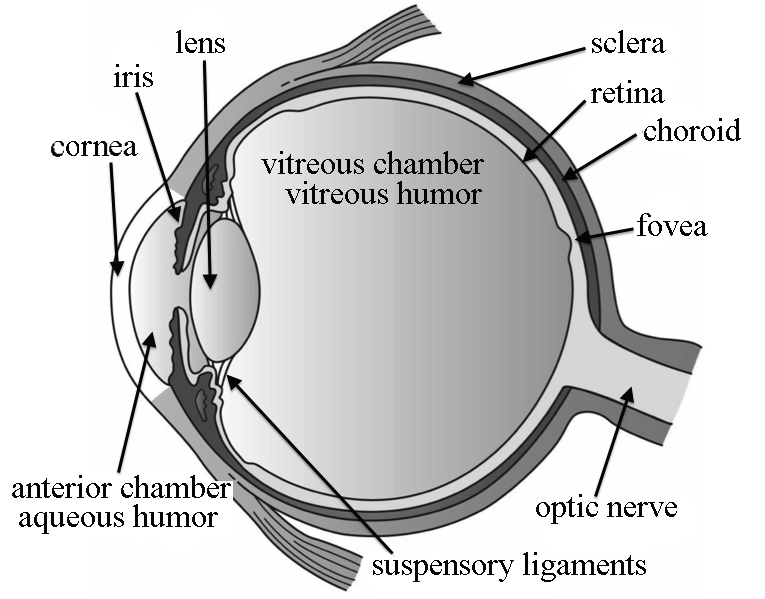
\includegraphics[width = 0.55\textwidth]{../../Figure/Other/Diagram of the human eye.png}
    \caption{Schema dell'occhio umano}
    \label{fig:1.1}
\end{wrapfigure}
Il concetto di visione artificiale è legato all'analisi di immagini digitali, nelle loro diverse caratteristiche.
Risulta dunque ovvio che comprendere come l'occhio umano percepisca ed elabori le immagini, risulti fondamentale.
Per quanto appena detto si descrive a seguire la struttura dell'occhio (\emph{Figura \ref{fig:1.1}}).

Questi é un'organo dalla forma pressoché sferica, si compone di diverse membrane delle quali di principale interesse è la retina.
Questa è la membrana più interna sulla quale sono disposti i \emph{fotocettori} responsabili della visione.
Tali fotocettori sono divisi in \emph{coni \emph{e} bastoncelli}: i primi in minor numero,
sono disposti attorno la fovea e sono responsabili della visione a colori,
i secondi presenti sull'intera superficie della retina sono responsabili della visone a scale di grigio.
\begin{Remark*}
    da quanto detto circa i fotocettori presenti nell'occhio umano,
    ne risulta che gli esseri umani sono molto più sensibili a variazioni di luce che non di colore.
\end{Remark*}

\begin{Remark*}
    per quanto concerne la visione a colori, si tenga presente che l'occhio umano è maggiormente sensibile, nell'ordine, a variazioni di verde, rosso e blu.
\end{Remark*}
\end{document}